% intro
In this section a background is given on the relevant concepts and techniques used in order to implement GP-CEPS. It is divided into four parts, namely controllable rare events, Neural Networks, Gaussian Processes and co-evolution. 

\subsection{Controllable Rare Events}
Figure \ref{rareControllableImage} illustrates the concept of controllable rare events with two policies. Rare events are defined as events that only occur in a small subset of episodes, while an event is controllable when the reward in an episode where the event occurred greatly depends on the policy chosen. A controllable rare event is thus an event of which the probability of occurring is low while the chosen policy significantly influences the reward.

\begin{figure}[ht]
  \centering
  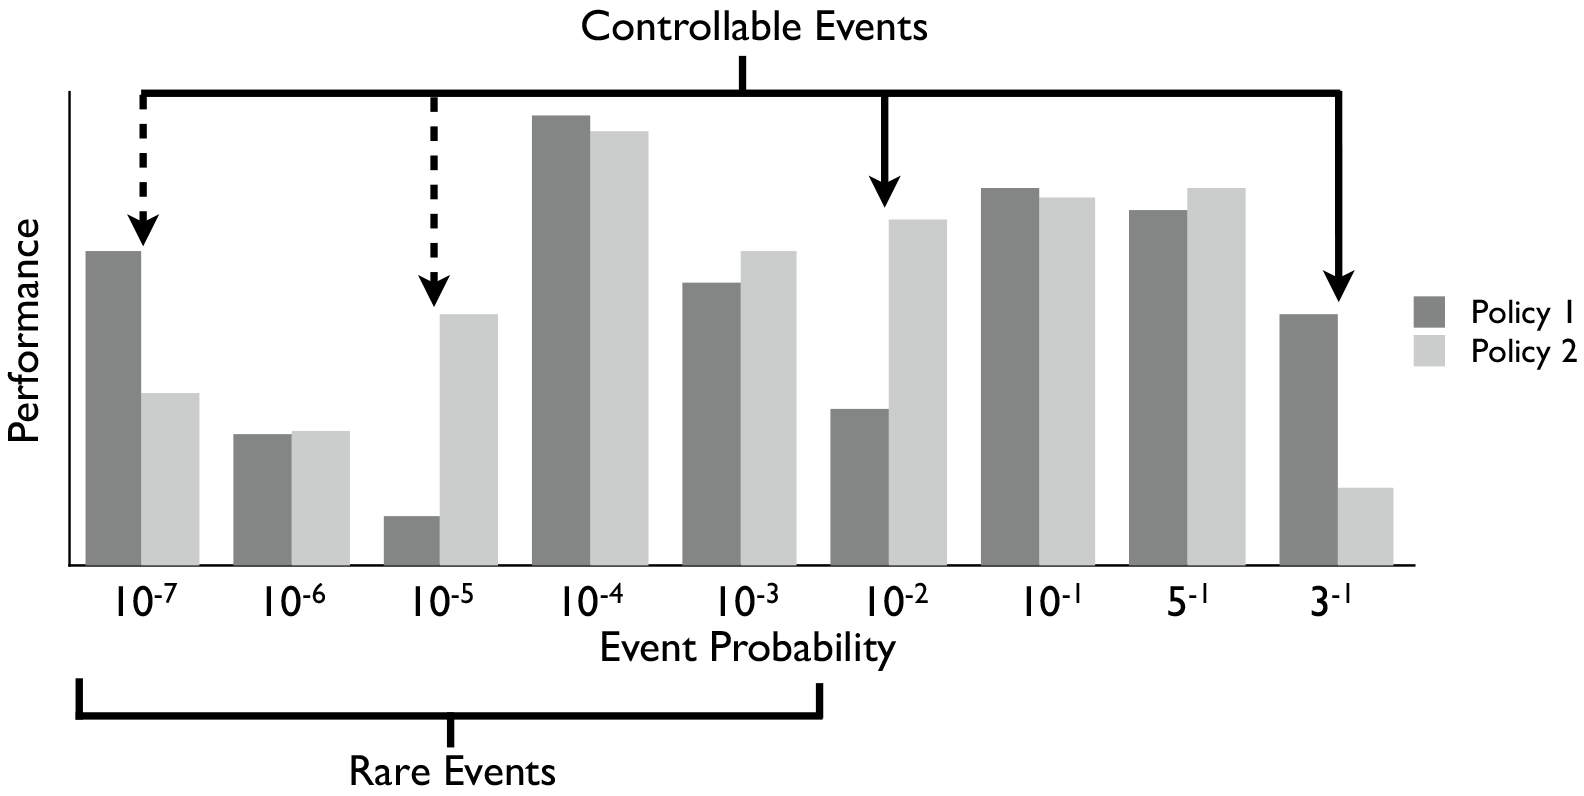
\includegraphics[scale=0.5]{images/rare-controllable.png}
  \caption{Performance of two policies on a set of events, showing rare-, controllable- and rare controllable events}\label{rareControllableImage}
\end{figure}

Dealing properly with events that are both rare and controllable is vital, because these events influence the performance of policies disproportionately while being difficult to train: general approaches tend to ignore rare events. By explicitly focusing on controllable rare events, policies with seemingly equal performance are properly distinguished and the learning process is accelerated.

\subsection{Neural Networks}
% meer in detail propagation uitleggen, or bias
Neural networks are inspired by the central nervous systems and are formed by layers of nodes, where each node in a layer has an activation function over the input times weights plus a bias \cite{bishop1995neural}. The activation function could for example be a hyperbolic tangent function. This would lead to:

\begin{align}
	\mbox{Output} = \tanh (\textbf{W} \textbf{x} + \textbf{b})
\end{align}

Nodes can be of three types: input-, output- or hidden nodes. The input nodes receive a signal (value), which are propagated to the next layer of nodes by multiplication with the corresponding weights. The values are propagated through the hidden layers and eventually reach the output nodes, which defines the output of the network. The input layer has dimensionality of the amount of features by the amount of hidden units, while the output layer has dimension amount of hidden units by the form of the output. For example in digits classification this is 10, one dimension for each digit.

Neural networks are viable options as representation for policies. In such a situation the input of the network is often the state of the world, while the output describes the action taken (given this state).

\subsection{Gaussian Process}
A Gaussian process is defined as a probability distribution over functions y(x) such that the set of values of y(x) evaluated at an arbitrary set of points $x_1, \dots, x_n$ jointly have a Gaussian distribution. \cite{bishop2006pattern} It can be used to do a regression and make predictions about new data points. This prediction is itself a Gaussian distribution, with a mean and a variance.

The GP has four hyper-parameters $\theta_1, \dot, \theta_4$ and a kernel that need to be set according to the input. From \ref{gp}, it becomes clear how important the hyper-parameters are. We see samples from the following (squared exponential) Gaussian kernel function prior:

\begin{align}
	k(\textbf{x}_n,\textbf{x}_m) = \theta_0 \exp \left \{ -\frac{\theta_1}{2} ||\textbf{x}_n-\textbf{x}_m ||^2 \right \} + \theta_2 + \theta_3\textbf{x}_n^T\textbf{x}_m
\end{align}

\begin{figure}[ht]
  \centering
  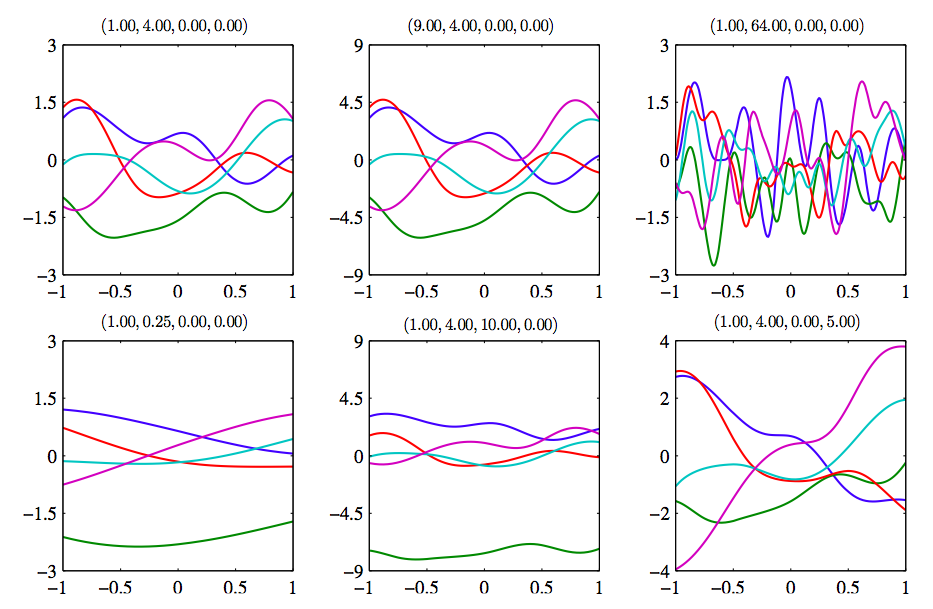
\includegraphics[scale=0.5]{images/gp.png}
  \caption{Sensitivity on the hyper-parameters \cite{bishop2006pattern}}\label{gp}
\end{figure}

\subsection{Co-Evolution}
% our context -> evolution bridge
Evolutionary Algorithms are used as a search method for the direct policy search. These algorithms aim to produce new entities based on a population and is inspired by biological evolution. Given a set of organisms, offspring is born by applying crossover and mutation operators, by combining the genes of the parents the new individuals exhibit similar, but slightly different, features. The selection of parents is based on an evaluation of the original set of organisms, and the better performing offspring replaces the least suited parents. In our case the policy is defined as a Neural Netowrk, so the set of weights of the network represents one organism in the population. The weights are then evolved as described above.

% co evolution 
Co evolution is the act of evolving two populations while their evaluation depends on the other population. A classical example is in a prey-predator context. The fitness of an individual depends on its survivability (either ability to hunt prey or evade predators) and the more fit a parent is, the more likely it produces offspring. This is often used to focus on evolving controllable rare events in combination with a good policy. A more detailed description of this will be given in the section on related work.

